\section{Evaluering}

\subsection{Observationer}

\begin{frame}
\frametitle{Punkter fra rapporten}
\begin{itemize}
\item Roterer og kører ikke præcist
\item Holder sig ikke altid indenfor den planlagte rute
\item Tager ikke højde for placering af sin bagende (og forende)
\item Sletter dele af kortet grundet forkerte sensormålinger
\item Uendelig løkke
\item Kører ind i forhindringer
\end{itemize}
\end{frame}

\subsection{Test af sensormodeller}
\begin{frame}
\frametitle{Sammenlignings-skema}
\begin{columns}
\begin{column}{.59\textwidth}
\begin{center}
\includegraphics[width=0.8\textwidth]{testresultater/emptygrid}\\
\begin{tabular}{ l l | c | c | c |}
\cline{3-5}
&&\multicolumn{3}{| c |}{Optimalt}\\\cline{3-5}
&& Optaget&Fri&Ukendt\\\hline

\multicolumn{1}{| l |}{\multirow{3}{*}{Test}}&
Optaget & $+1$ & {\color{red}$-1$} & {\color{gray}$0$}
\\\cline{2-5}

\multicolumn{1}{|c|}{}&
Fri     & {\color{red}$-1$} & $+1$ & {\color{gray}$0$}
\\\cline{2-5}

\multicolumn{1}{|c|}{}&
Ukendt  & {\color{red}$-1$} & {\color{red}$-1$} & {\color{gray}$0$}
 \\\hline
\end{tabular}
\end{center}
\end{column}
\begin{column}{.40\textwidth}
\visible<2->{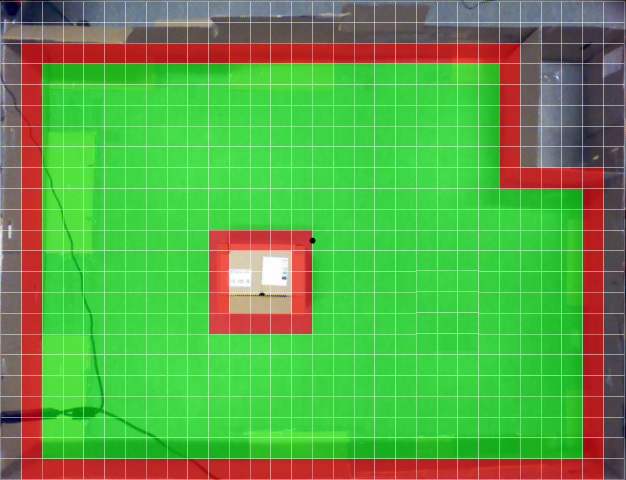
\includegraphics[width=\textwidth]{testresultater/optimalt}}\\
\visible<3->{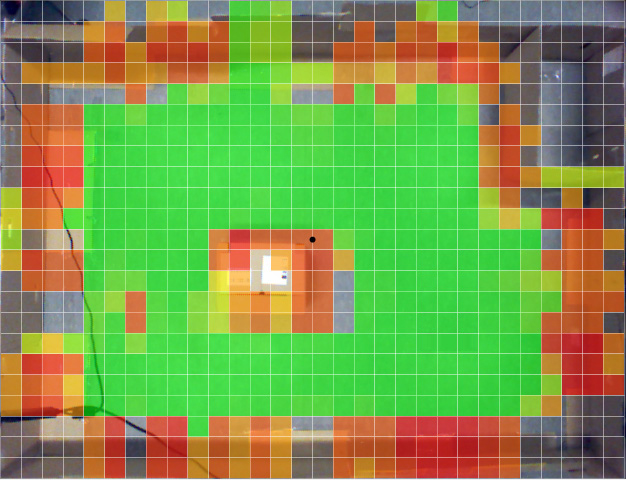
\includegraphics[width=\textwidth]{testresultater/simpel1}}
\end{column}
\end{columns}
\end{frame}

\begin{frame}
\frametitle{Testresultater}
\begin{columns}
\begin{column}{.59\textwidth}
\begin{center}
\begin{tabular}{|l|r|}
\hline
\textbf{Test \#} & \textbf{Resultat} \\ \hline \hline
Optimalt & 555 \\ \hline \hline
Simpel, Test 1 & 193 \\ \hline
Simpel, Test 2 & 187 \\ \hline
Simpel, Test 3 & 193 \\ \hline \hline
Gaussisk, Test 1 & 297 \\ \hline
Gaussisk, Test 2 & 325 \\ \hline
Gaussisk, Test 3 & 337 \\ \hline
\end{tabular}
\end{center}
\end{column}
\begin{column}{.40\textwidth}
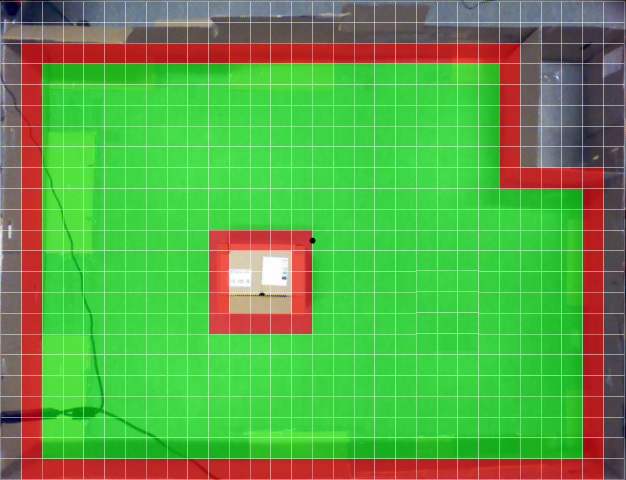
\includegraphics[width=\textwidth]{testresultater/optimalt}\\
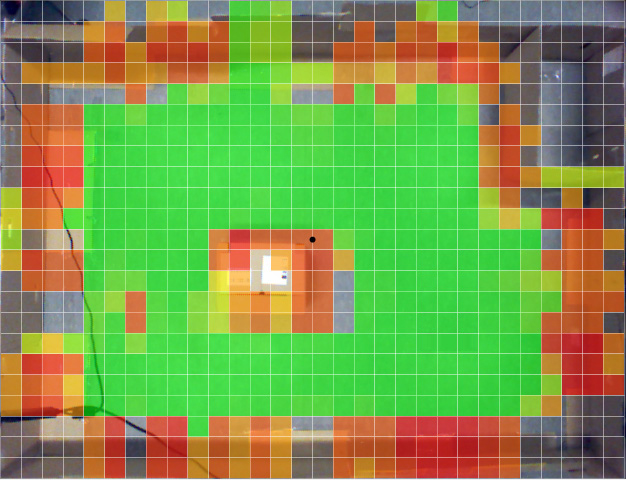
\includegraphics[width=\textwidth]{testresultater/simpel1}
\end{column}
\end{columns}
\end{frame}